In this section, we discuss the performance of \pred\ with respect to an increasing attention heads for the transformer model for the non-linear feedback model. Again note that the number of tasks $\Mpr \gg A \geq n$.
%
% Finally recall that when the horizon is small the weak demonstrator $\pi^w$ does not have sufficient samples for each action. This leads to a poor approximation of the greedy action. 
%
Through this experiment, we want to evaluate the performance of \pred\ to exploit the underlying reward correlation when the horizon is small and understand the representative power of the transformer by increasing the attention heads.
%
Note that we choose the non-linear feedback model and low data regime to leverage the representative power of the transformer.


\textbf{Baselines:} We again implement the same baselines discussed in \Cref{sec:short-horizon}. The baselines are \pred, \predt, \dptg, \ad, \ts, and \linucb. 


\textbf{Outcomes:} We first discuss the main outcomes of our experimental results for increasing the horizon:

% \noindent
% \textbf{(1)} The \pred\ (\gt) learns to exploit the underlying latent structure and reward correlation between the different tasks even when $A \geq n$ but $\Mpr \gg A$.

% \textbf{(2)} The \pred\ (\gt) has lower regret than its weak demonstrator even when trained on $\Dtr\subseteq\Dpr$.

% \textbf{(3)} The \pred\ (\gt) has lower regret compared to \dptg, \ad\ with increasing attention heads.

\begin{tcolorbox}
\customfinding \pred\ (\gt) outperforms \dptg, and \ad\ with increasing attention heads.
\end{tcolorbox}

% \begin{figure}[!hbt]
% \centering
% \begin{tabular}{ccc}
% \subfigure[Attention Heads $2$]{\hspace*{-1.8em}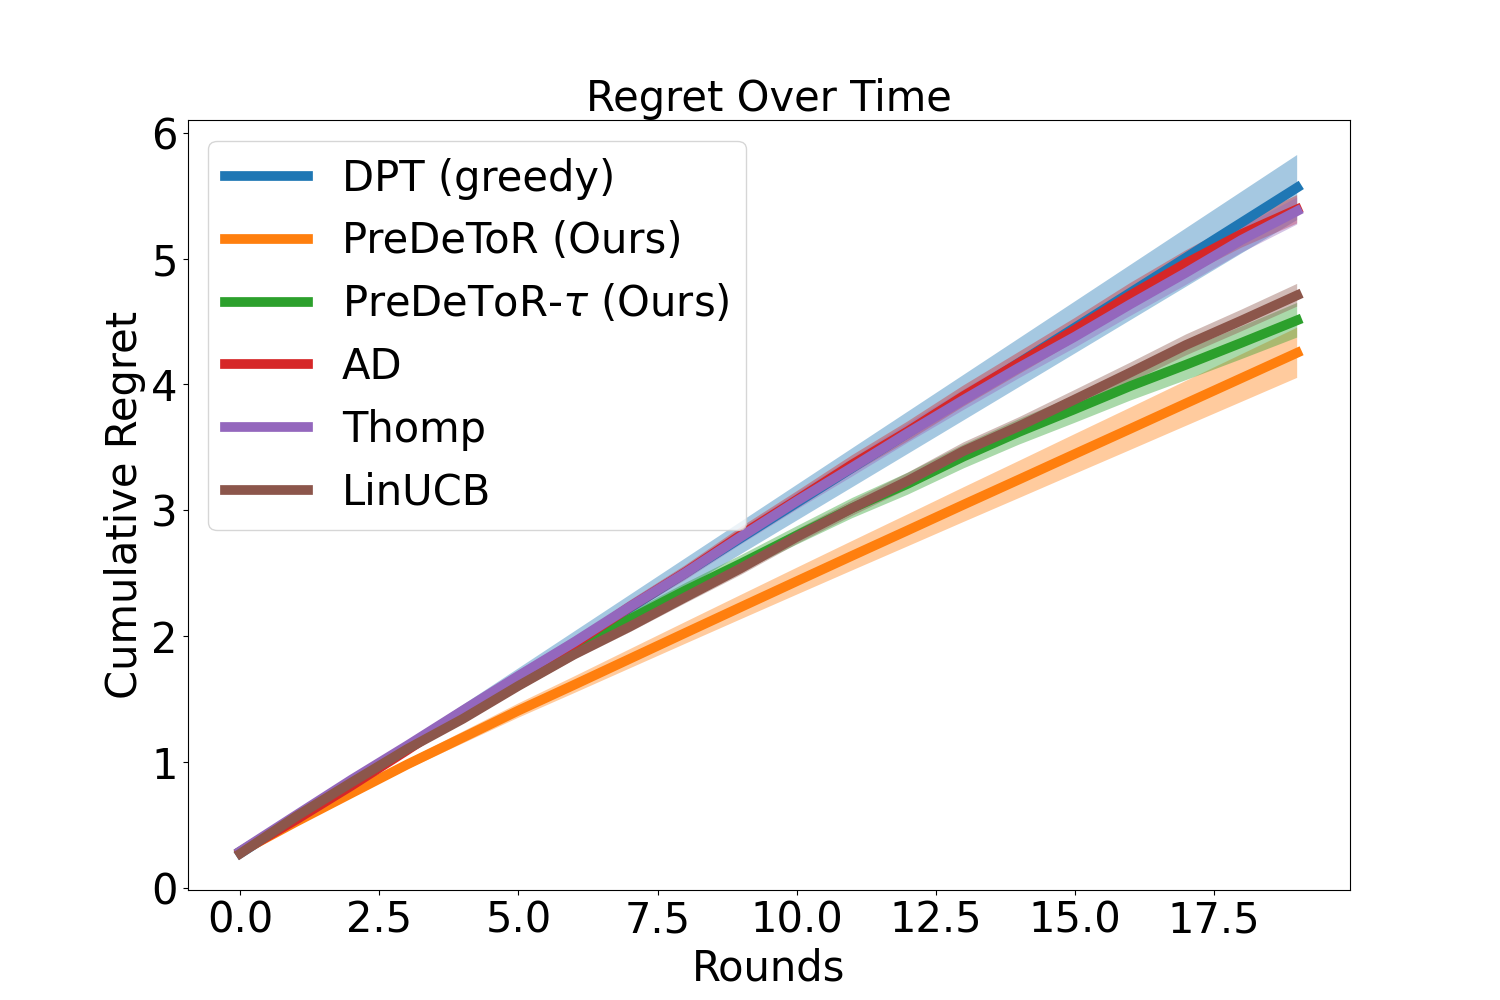
\includegraphics[scale = 0.13]{img/Neurips/head/lin_h2_lr0.00015_do0_embd32_layer2_head2_envs160000_hists1_samples1_var0.3_cov0.0_H20_d20_lind40_seed1_testcov0.0_hor20.pkl.png}\label{fig:head-2}} &
% %%%%%%%%%%
% \subfigure[Attention Heads $4$]{\hspace*{-1.8em}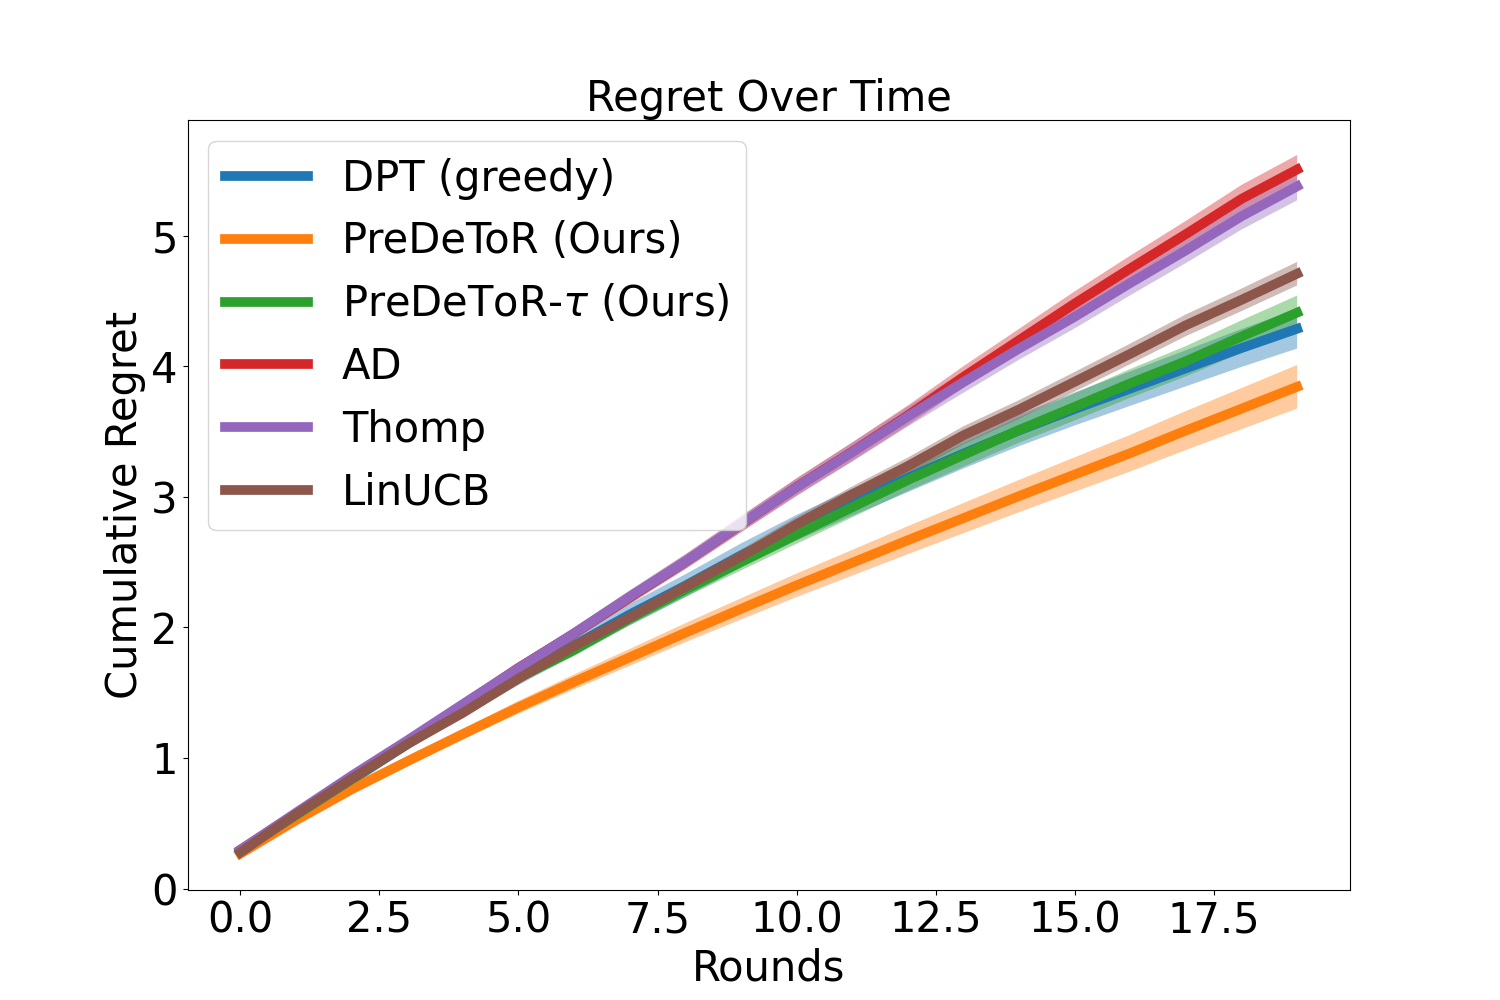
\includegraphics[scale = 0.13]{img/Neurips/head/lin_h4_lr0.00015_do0_embd32_layer4_head4_envs160000_hists1_samples1_var0.3_cov0.0_H20_d20_lind40_seed1_testcov0.0_hor20.pkl.png} \label{fig:head-4}} &
% %%%%%%%%%%%%%%%%%%%%%%%
% \subfigure[Attention Heads $6$]{\hspace*{-1.8em}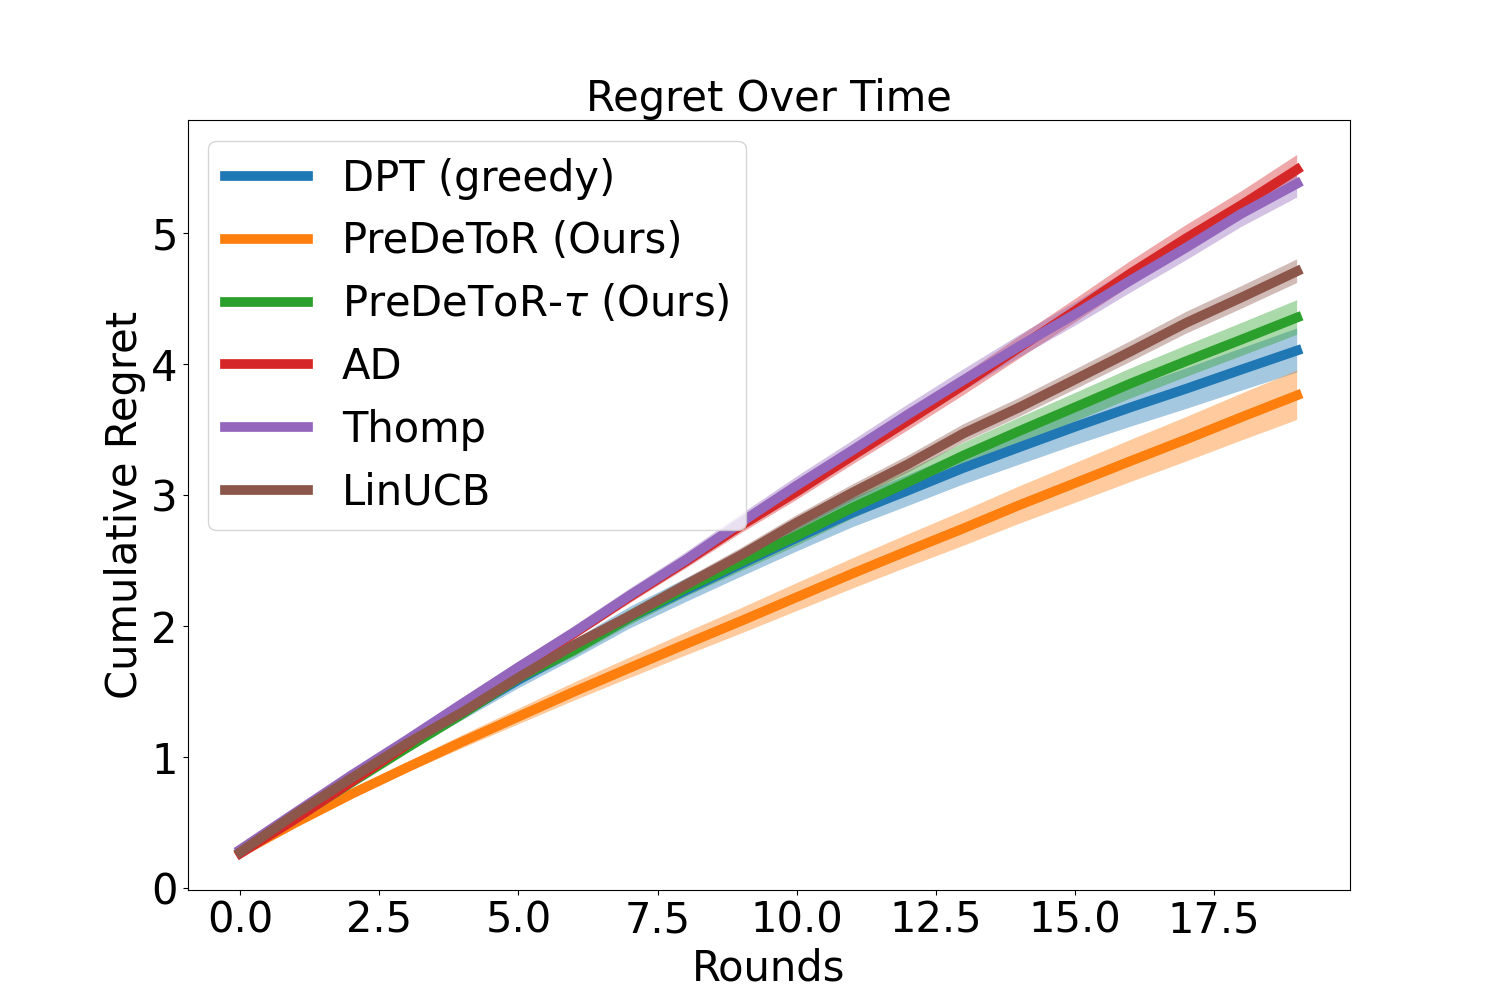
\includegraphics[scale = 0.13]{img/Neurips/head/lin_h6_lr0.00015_do0_embd32_layer6_head6_envs160000_hists1_samples1_var0.3_cov0.0_H20_d20_lind40_seed1_testcov0.0_hor20.pkl.png}\label{fig:head-6}} \\
% % \end{tabular}
% % \begin{tabular}{cc}
% %%%%%%%%%%
% \subfigure[Attention Heads $8$]{\hspace*{-1.8em}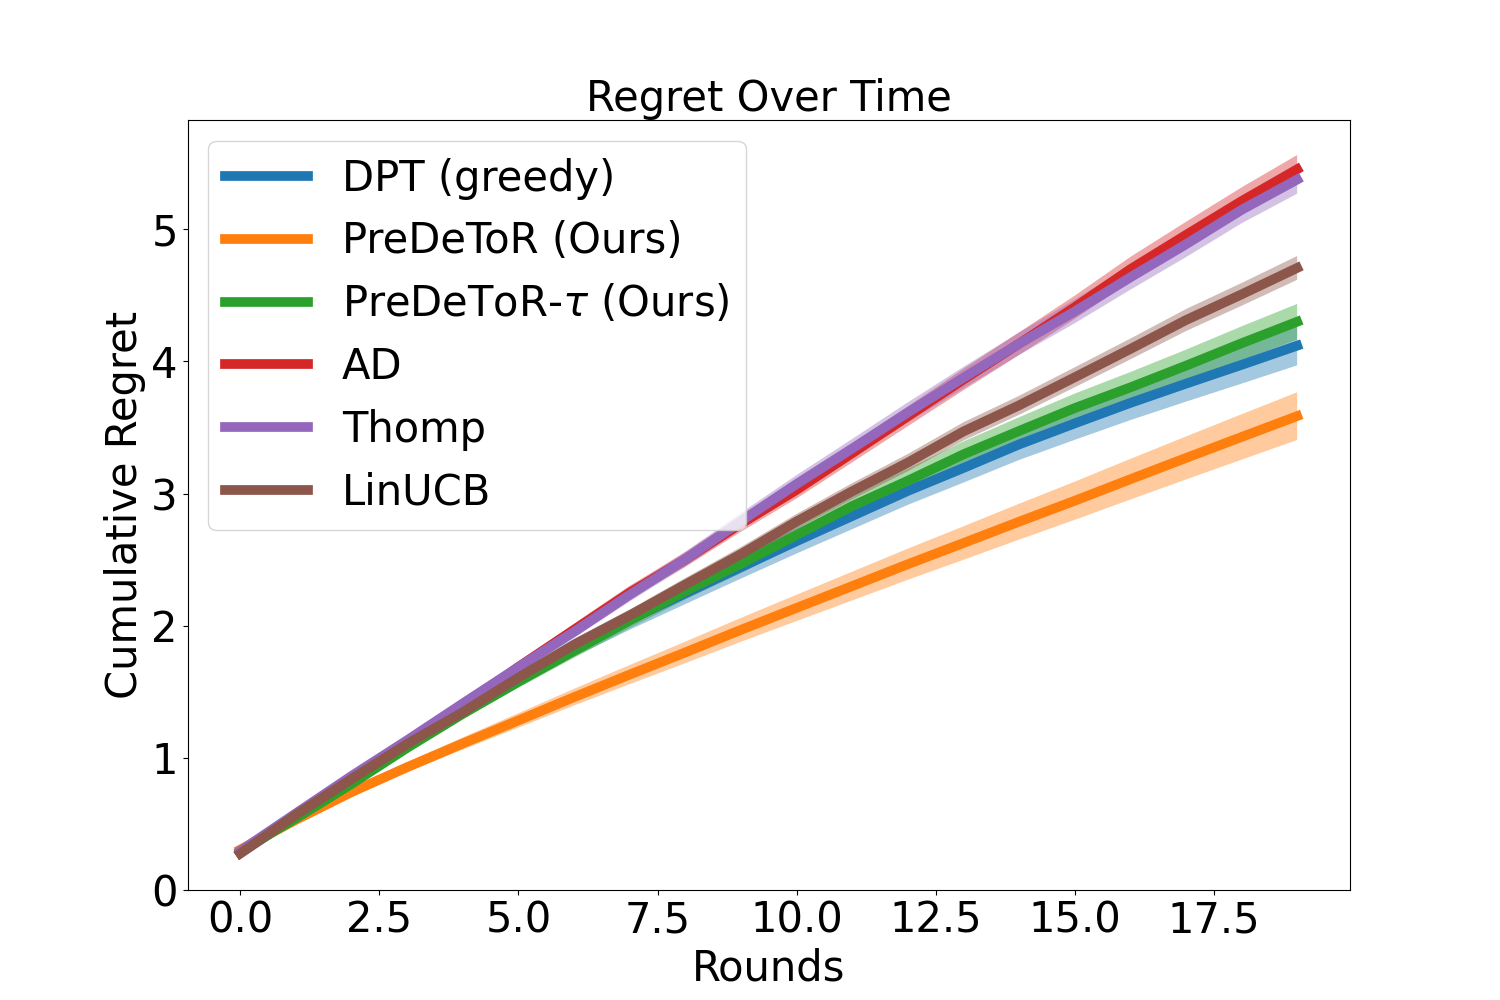
\includegraphics[scale = 0.13]{img/Neurips/head/lin_h8_lr0.00015_do0_embd32_layer8_head8_envs160000_hists1_samples1_var0.3_cov0.0_H20_d20_lind40_seed1_testcov0.0_hor20.pkl.png} \label{fig:head-8}} &
% %%%%%%%%%%%%%%%%%%%%%%%%%%%%%%%%
% \subfigure[Attention Heads $12$]{\hspace*{-1.8em}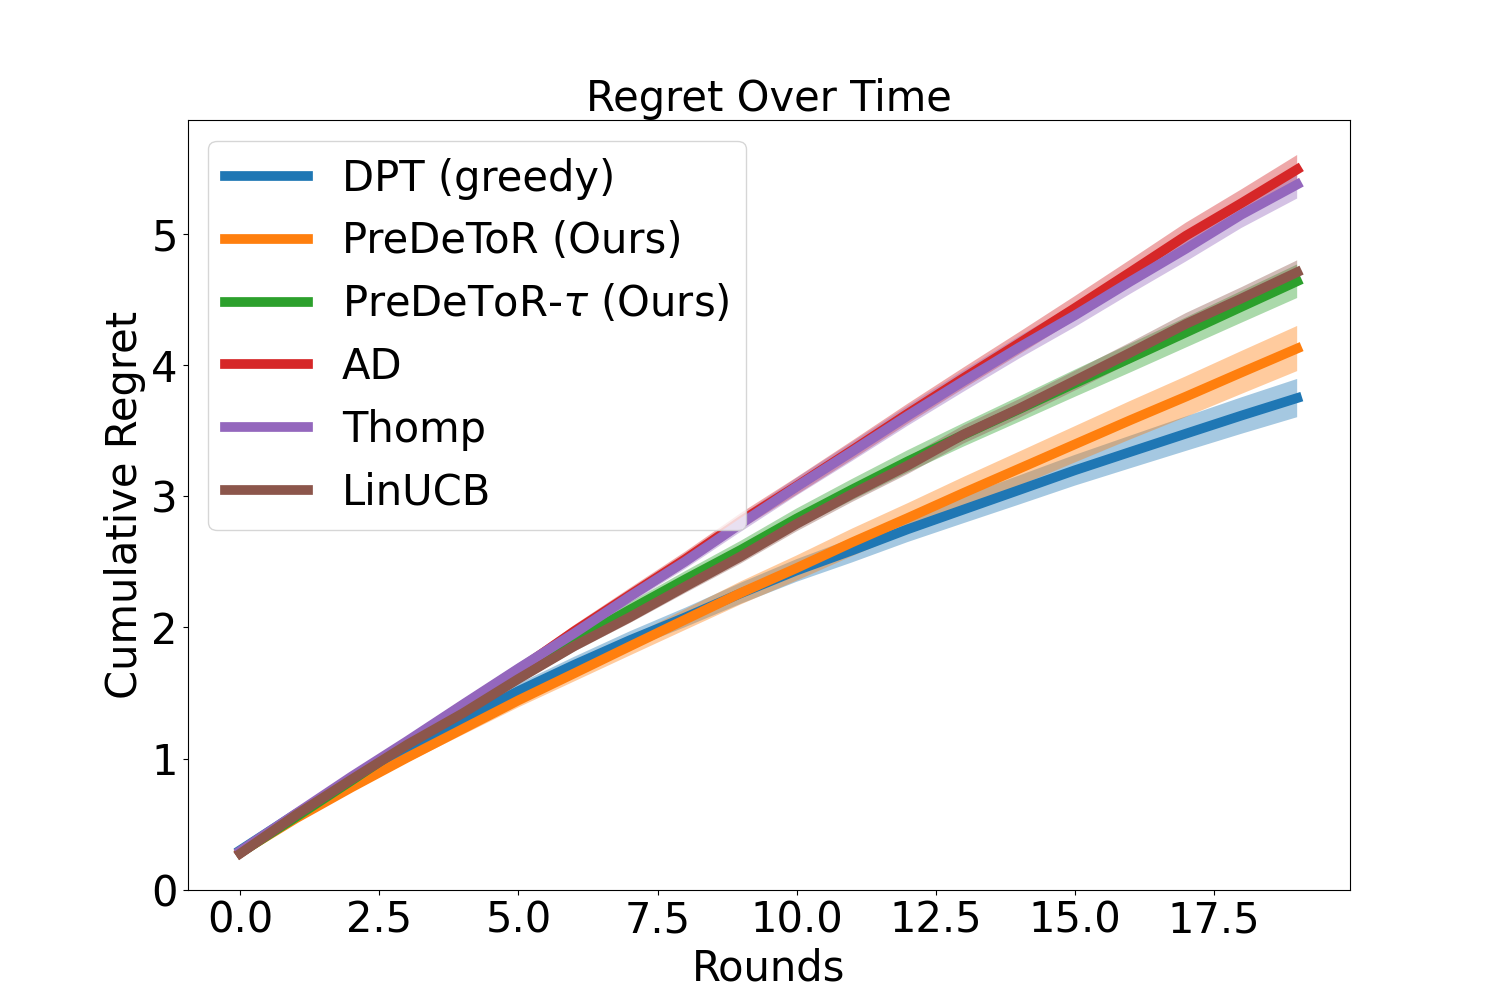
\includegraphics[scale = 0.13]{img/Neurips/head/lin_h12_lr0.00015_do0_embd32_layer12_head12_envs160000_hists1_samples1_var0.3_cov0.0_H20_d20_lind40_seed1_testcov0.0_hor20.pkl.png} \label{fig:head-12}} &
% %%%%%%%%%%%%%%%%%%%%%%%%%%%%%%%
% \subfigure[Increasing Attention Heads]{\hspace*{-1.8em}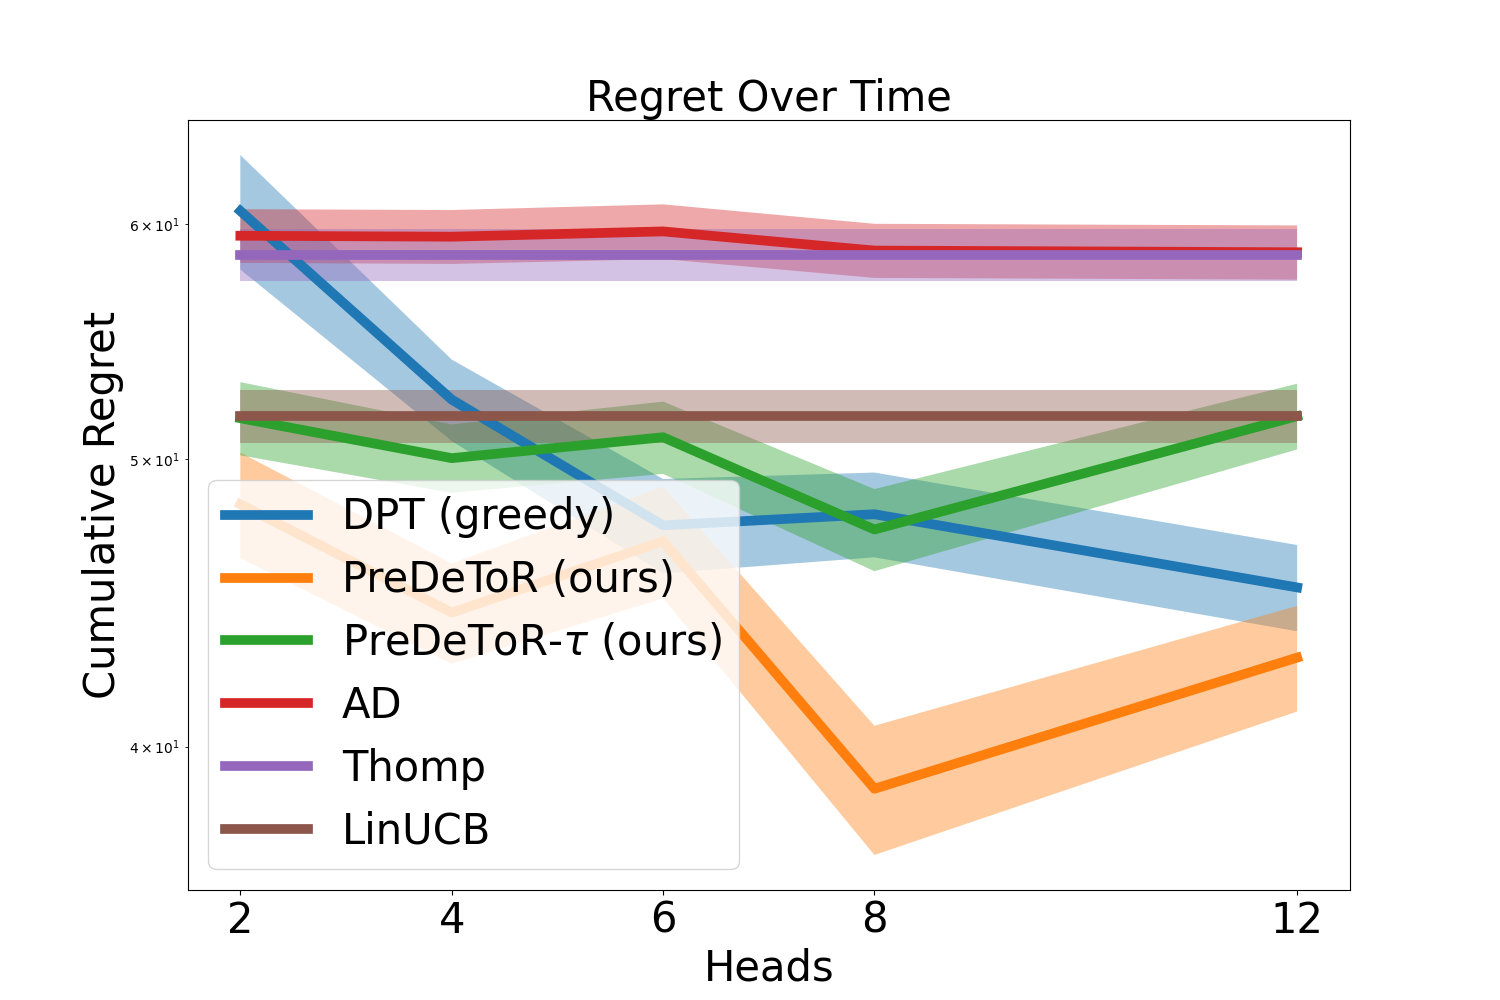
\includegraphics[scale = 0.13]{img/Neurips/head/heads_fig.png} \label{fig:head-inc}}
% \end{tabular}
% \vspace*{-1em}
% \caption{Experiment with increasing attention heads. The y-axis shows the cumulative regret.}
% \label{fig:expt-head}
% \vspace{-0.7em}
% \end{figure}

\begin{figure}[!hbt]
\centering
\begin{subfigure}[b]{0.32\textwidth}
   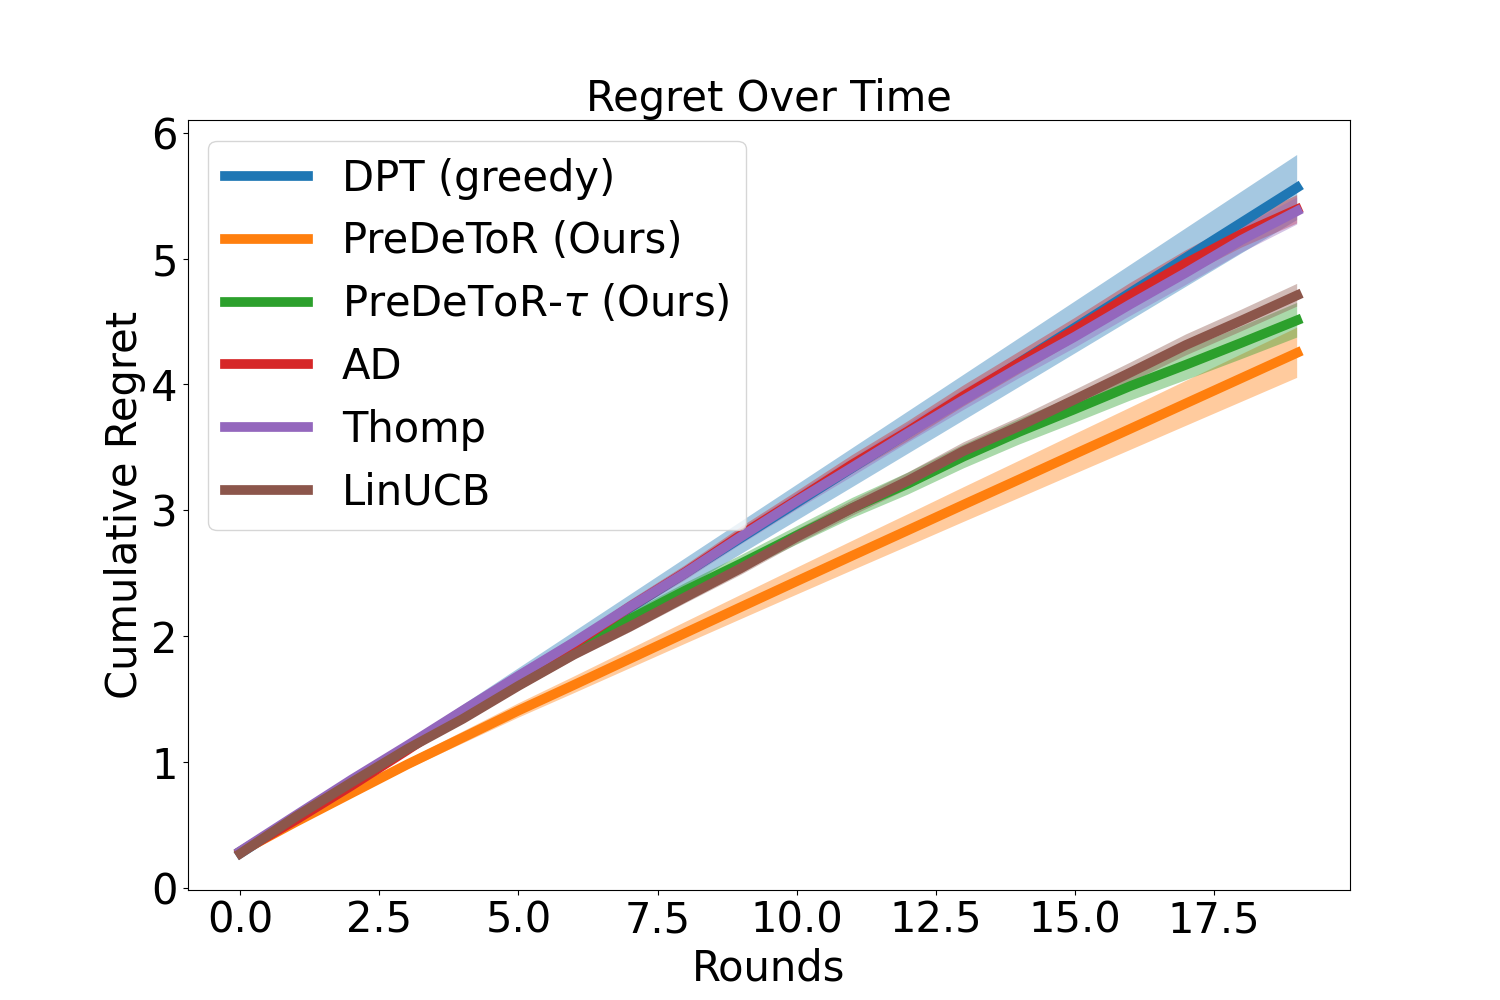
\includegraphics[scale=0.13]{img/Neurips/head/lin_h2_lr0.00015_do0_embd32_layer2_head2_envs160000_hists1_samples1_var0.3_cov0.0_H20_d20_lind40_seed1_testcov0.0_hor20.pkl.png}
   \caption{Attention Heads $2$}
   \label{fig:head-2}
\end{subfigure}%
\begin{subfigure}[b]{0.32\textwidth}
   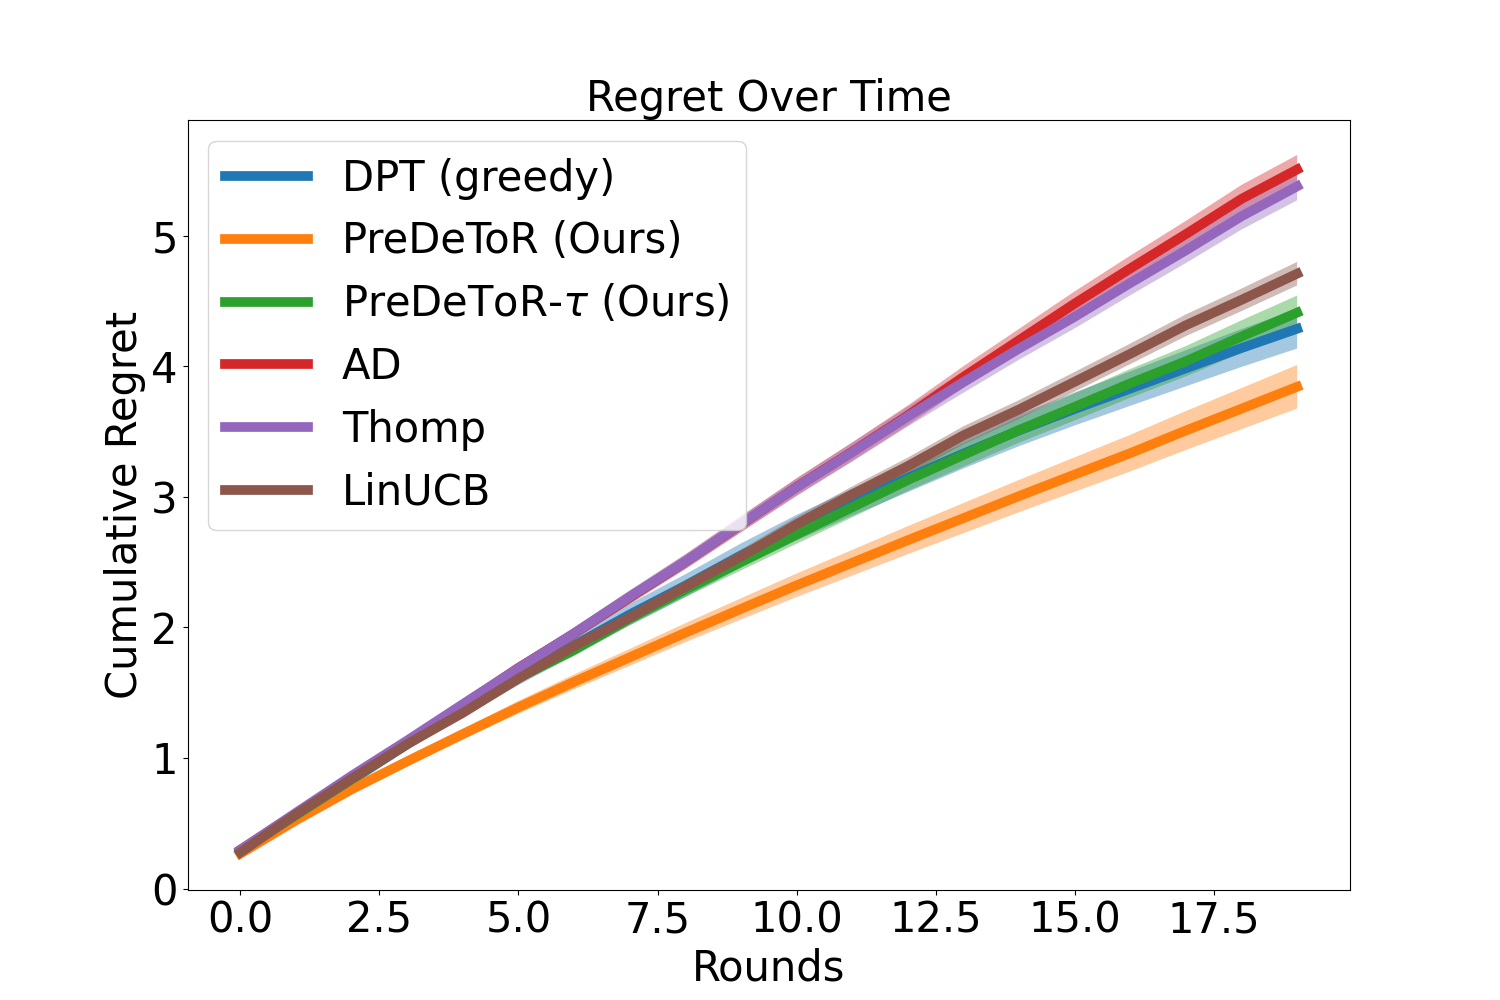
\includegraphics[scale=0.13]{img/Neurips/head/lin_h4_lr0.00015_do0_embd32_layer4_head4_envs160000_hists1_samples1_var0.3_cov0.0_H20_d20_lind40_seed1_testcov0.0_hor20.pkl.png}
   \caption{Attention Heads $4$}
   \label{fig:head-4}
\end{subfigure}%
\begin{subfigure}[b]{0.32\textwidth}
   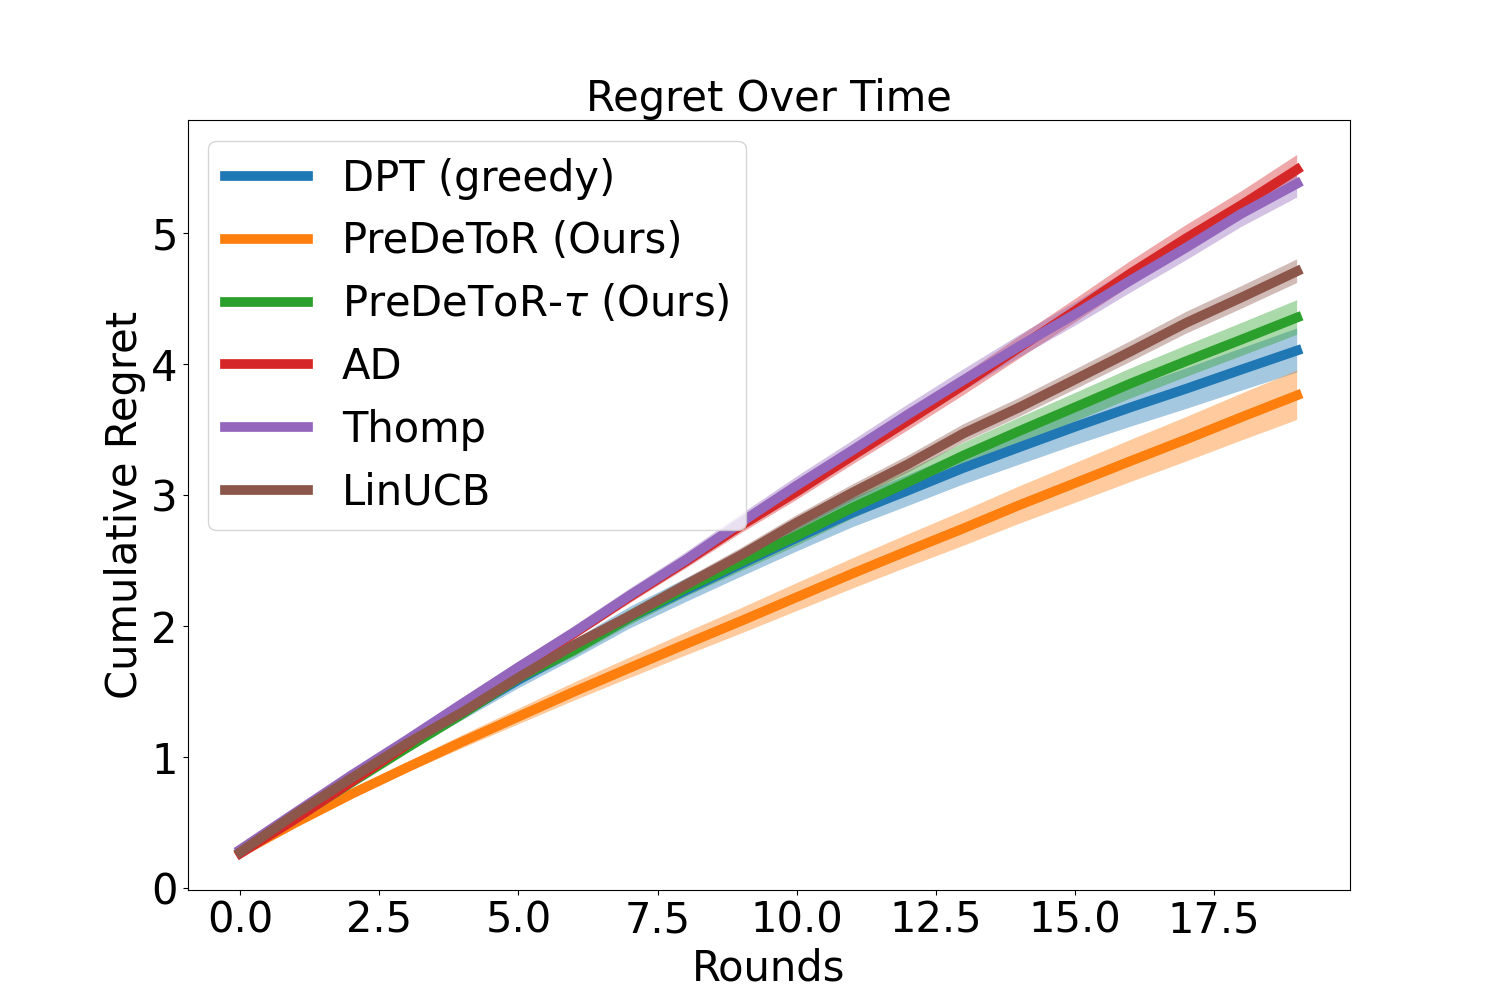
\includegraphics[scale=0.13]{img/Neurips/head/lin_h6_lr0.00015_do0_embd32_layer6_head6_envs160000_hists1_samples1_var0.3_cov0.0_H20_d20_lind40_seed1_testcov0.0_hor20.pkl.png}
   \caption{Attention Heads $6$}
   \label{fig:head-6}
\end{subfigure}

\begin{subfigure}[b]{0.32\textwidth}
   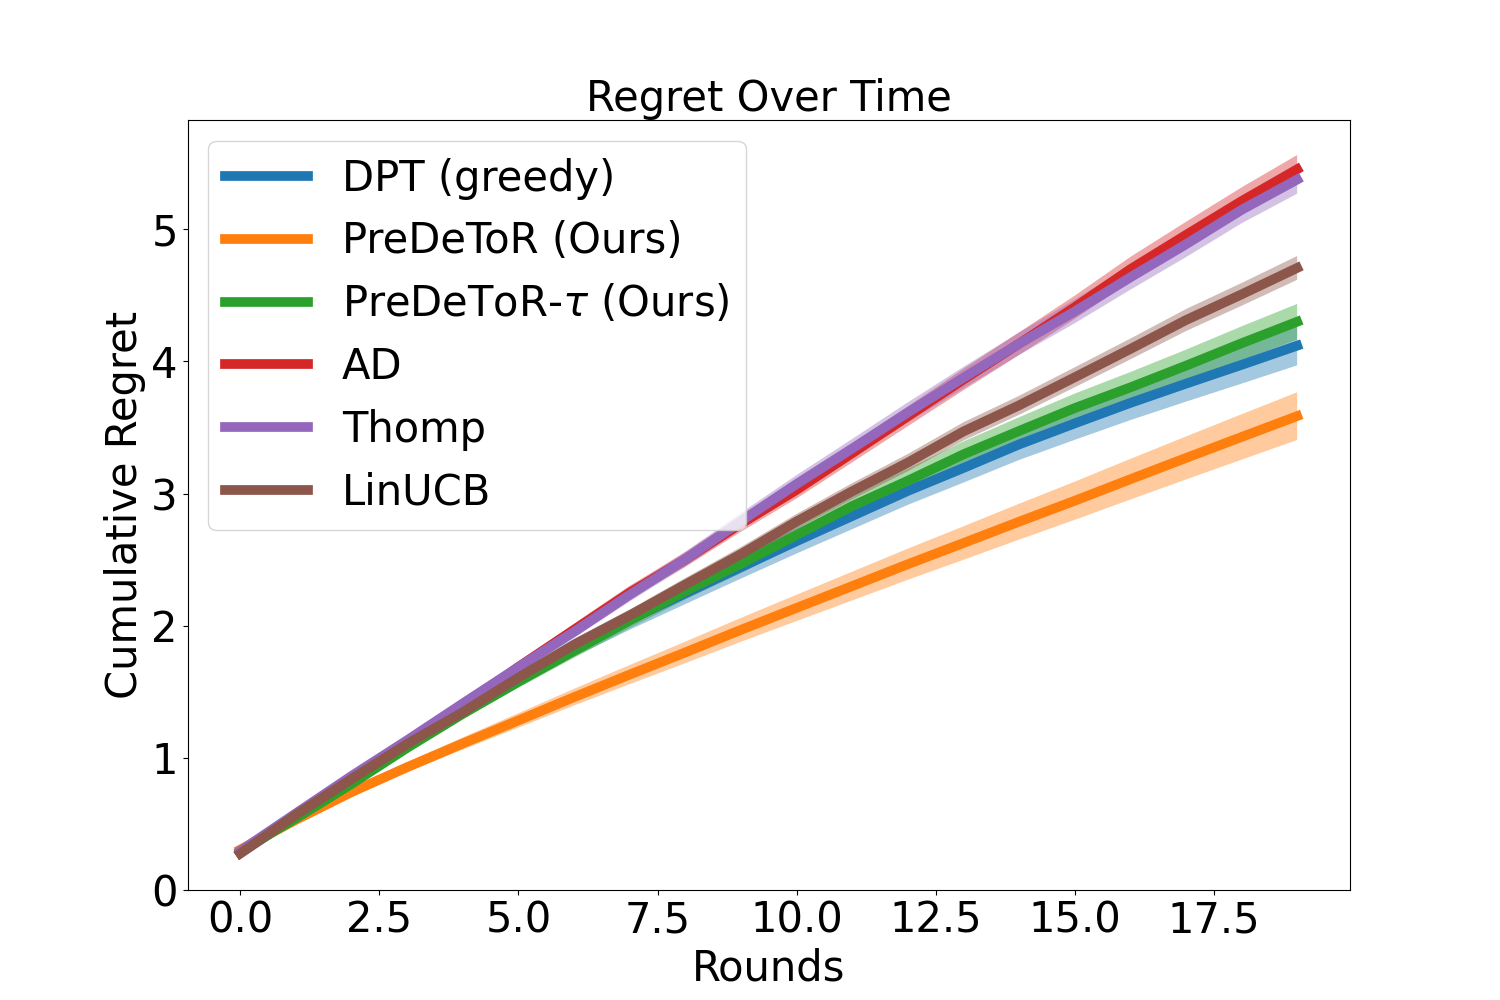
\includegraphics[scale=0.13]{img/Neurips/head/lin_h8_lr0.00015_do0_embd32_layer8_head8_envs160000_hists1_samples1_var0.3_cov0.0_H20_d20_lind40_seed1_testcov0.0_hor20.pkl.png}
   \caption{Attention Heads $8$}
   \label{fig:head-8}
\end{subfigure}%
\begin{subfigure}[b]{0.32\textwidth}
   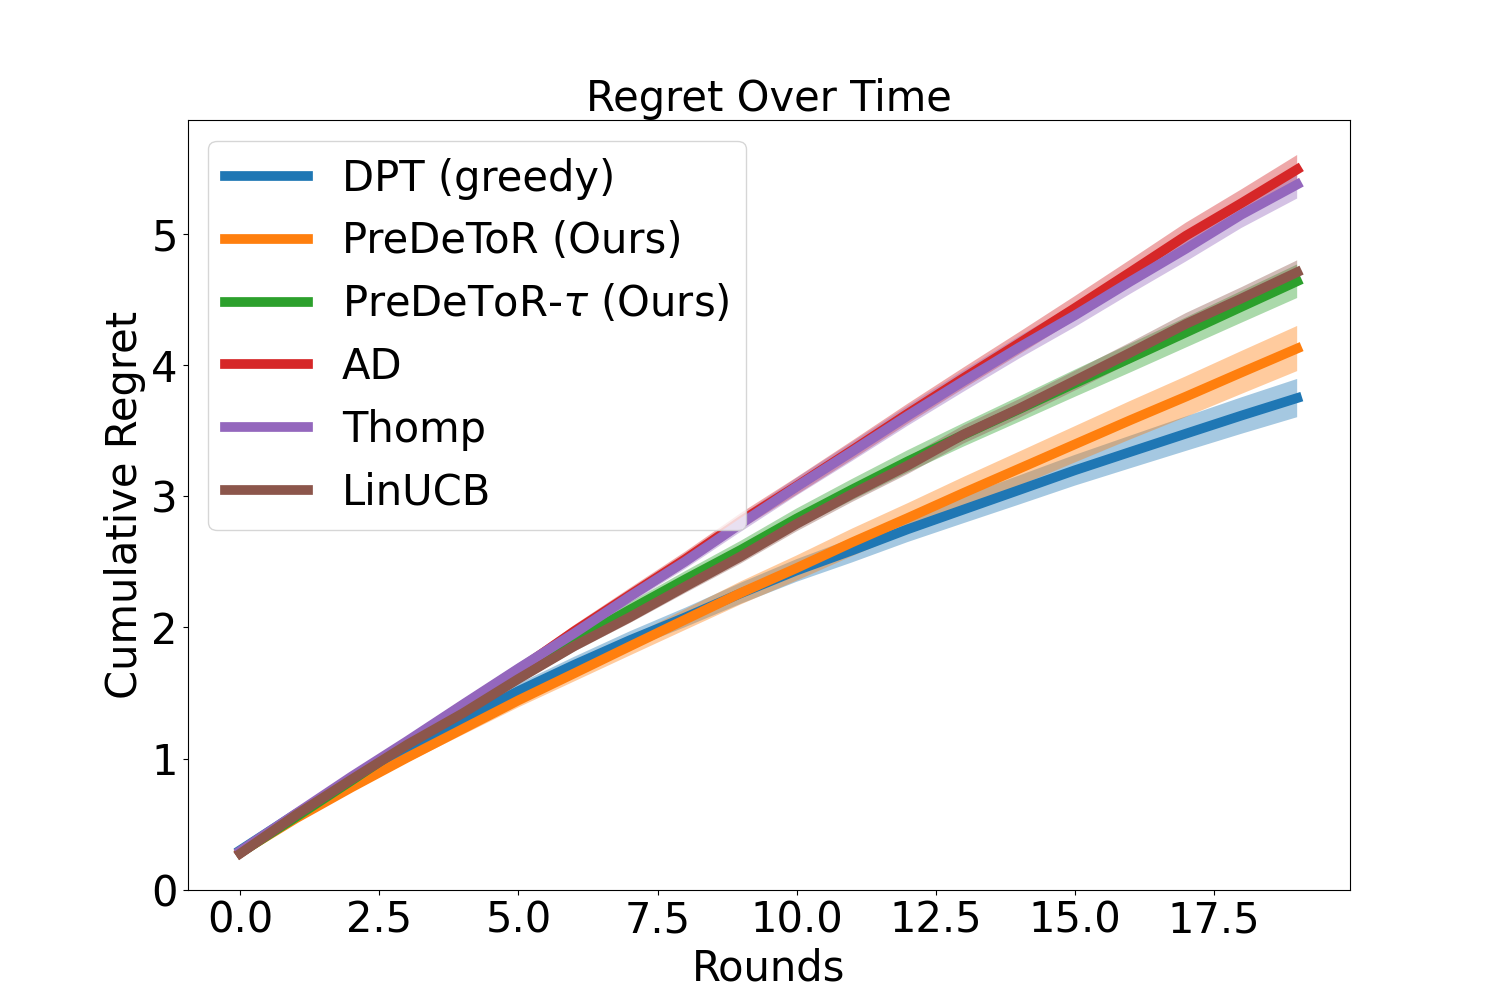
\includegraphics[scale=0.13]{img/Neurips/head/lin_h12_lr0.00015_do0_embd32_layer12_head12_envs160000_hists1_samples1_var0.3_cov0.0_H20_d20_lind40_seed1_testcov0.0_hor20.pkl.png}
   \caption{Attention Heads $12$}
   \label{fig:head-12}
\end{subfigure}%
\begin{subfigure}[b]{0.32\textwidth}
   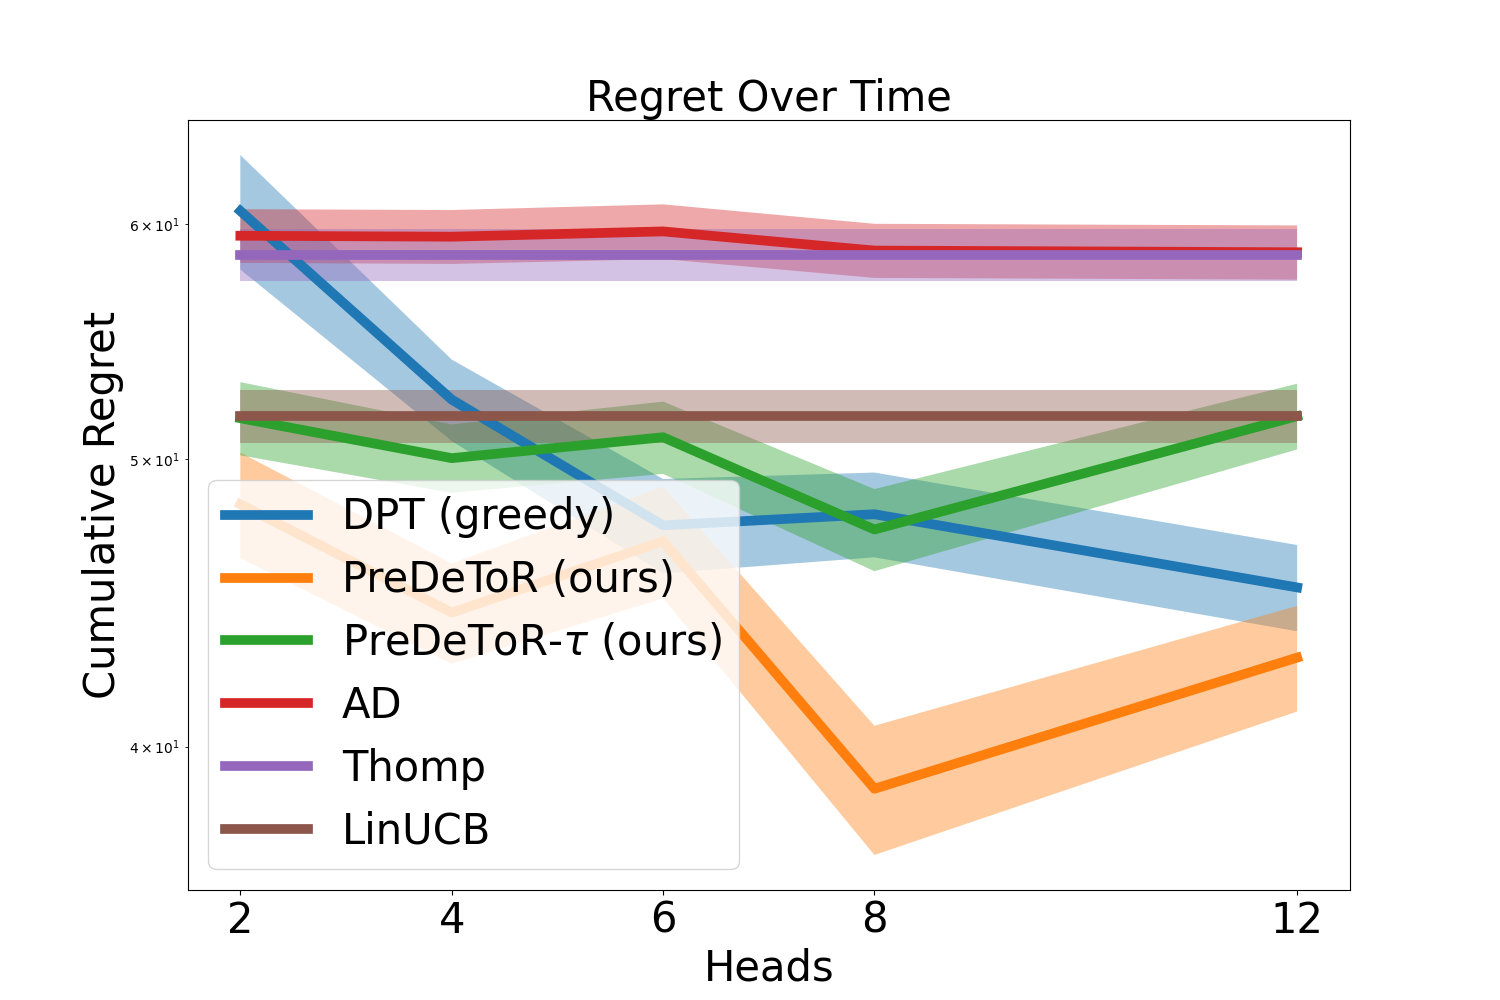
\includegraphics[scale=0.13]{img/Neurips/head/heads_fig.png}
   \caption{Increasing Attention Heads}
   \label{fig:head-inc}
\end{subfigure}
\vspace*{-1em}
\caption{Experiment with increasing attention heads. The y-axis shows the cumulative regret.}
\label{fig:expt-head}
\vspace{-0.7em}
\end{figure}

\textbf{Experimental Result:} We observe these outcomes in \Cref{fig:expt-head}. In \Cref{fig:expt-head} we show the non-linear bandit setting for horizon $n=20$, $\Mpr =  160000$, $\Mts = 200$, $A=20$, $\mathrm{heads}=\{2, 4, 6, 8\}$ and $d=5$. 
%
%
Again, the demonstrator $\pi^w$ is the \ts\ algorithm. We observe that \pred\ (\gt) has lower cumulative regret than \dptg, \ad. Note that for any task $m$ for the horizon $20$ the \ts\ will be able to sample all the actions atmost once.
% Moreover \pred\ matches the performance of \linucb. 
%
%The weak performance of \dptg\ can be attributed to both short horizons and the inability to estimate the optimal action for such a short horizon $H < A$. 
%
%Note that for this small horizon setting the \dptg\ does not have a good estimation of $\widehat{a}_{m,*}$ which results in a poor prediction of optimal action $\widehat{a}_{m,t,*}$. 
% This results in higher regret. 
Observe from \Cref{fig:head-2}, \ref{fig:head-4}, \ref{fig:head-6}, and \ref{fig:head-8} that \pred\ (\gt) has lower regret than \ad, \ts\ and \linucb\ which also shows that \pred\ (\gt) is exploiting the latent linear structure of the underlying tasks for the non-linear setting.
%
% The training of \ad\ ensures that it does not outperform the demonstrator \ts.
%
In \Cref{fig:head-inc} we plot the regret of all the baselines with respect to the increasing attention heads. Again we see that \pred\ (\gt) regret decreases as we increase the attention heads. 

% This shows that \pred\ training procedure is able to capture the reward correlation better and hence predict the reward of the optimal action more efficiently with different numbers of attention heads.